\documentclass[border=8pt]{standalone}
\usepackage{amsmath,amssymb,bm}
\usepackage{xcolor}
\usepackage{tikz}
\usetikzlibrary{arrows.meta}
\definecolor{ACC}{HTML}{D5772A}
\definecolor{ink}{HTML}{1B1B2F}
\begin{document}
\large
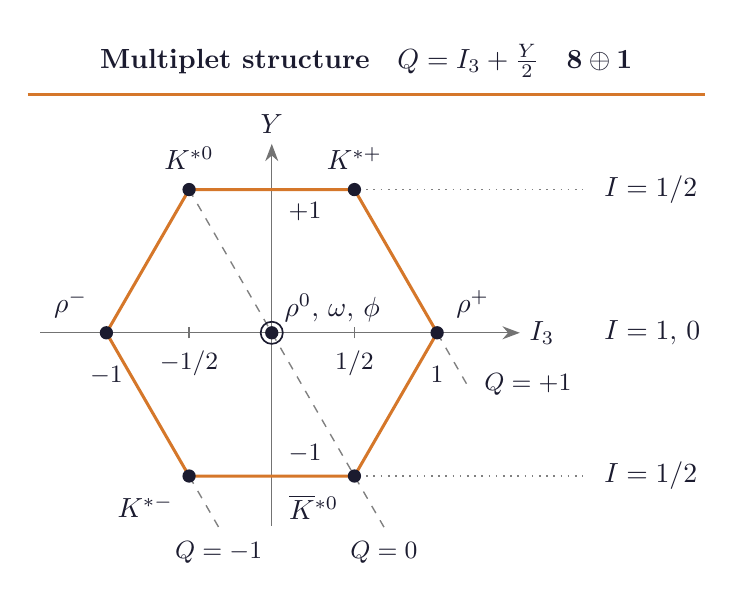
\begin{tikzpicture}[>=Stealth, every node/.style={text=ink}]
\path[use as bounding box] (-3.100,-3.025) rectangle (5.500,3.875);
\node at (1.200,3.45) {\textbf{Multiplet structure}\quad $Q=I_3+\tfrac{Y}{2}$\quad $\mathbf{8\oplus 1}$};
\draw[ACC,line width=.9pt] (-3.100,3.025) -- (5.500,3.025);
\draw[-{Stealth[length=2.2mm]},black!55,line width=.5pt] (-2.940,0) -- (3.150,0) node[right] {$I_3$};
\draw[-{Stealth[length=2.2mm]},black!55,line width=.5pt] (0,-2.45) -- (0,2.4) node[above] {$Y$};
\draw[black!55,line width=.5pt] (-2.100,-0.07) -- (-2.100,0.07); \node[anchor=north,font=\small] at (-2.100,-0.300) {$-1$};
\draw[black!55,line width=.5pt] (-1.050,-0.07) -- (-1.050,0.07); \node[anchor=north,font=\small] at (-1.050,-0.100) {$-1/2$};
\draw[black!55,line width=.5pt] (1.050,-0.07) -- (1.050,0.07); \node[anchor=north,font=\small] at (1.050,-0.100) {$1/2$};
\draw[black!55,line width=.5pt] (2.100,-0.07) -- (2.100,0.07); \node[anchor=north,font=\small] at (2.100,-0.300) {$1$};
\draw[black!55,line width=.5pt] (-0.07,1.819) -- (0.07,1.819); \node[anchor=north west,font=\small] at (0.09,1.779) {$+1$};
\draw[black!55,line width=.5pt] (-0.07,-1.819) -- (0.07,-1.819); \node[anchor=south west,font=\small] at (0.09,-1.779) {$-1$};
\draw[black!50,dashed,line width=.5pt] (1.050,1.819) -- (2.475,-0.650);
\node[anchor=west,font=\small] at (2.575,-0.650) {$Q=+1$};
\draw[black!50,dashed,line width=.5pt] (-1.050,1.819) -- (1.425,-2.468);
\node[anchor=north,font=\small] at (1.425,-2.528) {$Q=0$};
\draw[black!50,dashed,line width=.5pt] (-2.100,0.000) -- (-0.675,-2.468);
\node[anchor=north,font=\small] at (-0.675,-2.528) {$Q=-1$};
\draw[ACC,line width=1.1pt,line join=round] (1.050,1.819) -- (2.100,0.000) -- (1.050,-1.819) -- (-1.050,-1.819) -- (-2.100,0.000) -- (-1.050,1.819) -- cycle;
\fill[ink] (1.050,1.819) circle (2.4pt);
\fill[ink] (2.100,0.000) circle (2.4pt);
\fill[ink] (1.050,-1.819) circle (2.4pt);
\fill[ink] (-1.050,-1.819) circle (2.4pt);
\fill[ink] (-2.100,0.000) circle (2.4pt);
\fill[ink] (-1.050,1.819) circle (2.4pt);
\draw[ink,line width=.6pt] (0,0) circle (4pt); \fill[ink] (0,0) circle (2.4pt);
\node[anchor=south] at (1.050,1.949) {$K^{*+}$};
\node[anchor=south] at (-1.050,1.949) {$K^{*0}$};
\node[anchor=south west] at (2.220,0.070) {$\rho^+$};
\node[anchor=south east] at (-2.220,0.070) {$\rho^-$};
\node[anchor=north east] at (-1.130,-1.939) {$K^{*-}$};
\node[anchor=north east] at (0.970,-1.939) {$\overline{K}{}^{*0}$};
\node[anchor=south west,fill=white,inner sep=1pt] at (0.12,0.1) {$\rho^0,\,\omega,\,\phi$};
\draw[black!50,dotted,line width=.6pt] (1.200,1.819) -- (3.950,1.819);
\node[anchor=west] at (4.100,1.819) {$I=1/2$};
\node[anchor=west] at (4.100,0.000) {$I=1,\,0$};
\draw[black!50,dotted,line width=.6pt] (1.200,-1.819) -- (3.950,-1.819);
\node[anchor=west] at (4.100,-1.819) {$I=1/2$};
\end{tikzpicture}
\end{document}
